% Chapter 3

\chapter{Methodology and Tools} % Write in your own chapter title
\label{Chapter3}
\lhead{} % Write in your own chapter title to set the page header

\section{System Level Design}
\subsection{Application in Communication Systems}
Traditional methods for data recovery include channel estimation through the use of pilots. In that, LS estimation or MMSE is used. At first, we investigate the performance of Deep Learning architecture for a constant, single tap channel with white noise at specified SNR.   \\
Then, we increase the number of channel taps to 8 and make a Gaussian channel. By varying channel parameters and types (No of Channel Realizations, Fading or Non fading etc.), we repeat the analysis. \\
We then use DNN to recover data bits transmitted from two different users with non-orthogonal resource allocation, at a single receiver
\begin{figure}[htbp]
  \centering
  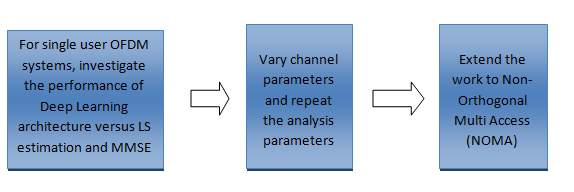
\includegraphics[width=\textwidth]{./Figures/comm_design.png}
  \caption{System level design for Communication Systems}
  \label{fig:comm_design}
\end{figure}
\subsection{Application in Bioinformatics}
Traditional methods for Parkinson's diagnosis involve a subjective clinical diagnosis. However, through the use of mPower data \cite{bot2016mpower}, we intend to augment that process with an easy-to-use predictive Neural Network architecture. We do that by understanding the data provided to us first and then apply Machine Learning techniques with hand-crafted people to generate initial results.\\
Then we replace those networks with more sophisticated Deep Learning Models and improve upon those results.\\
After that, we move towards End-to-End Deep Learning which removes all the steps required to prepare features for input to our model.
\begin{figure}[htbp]
  \centering
  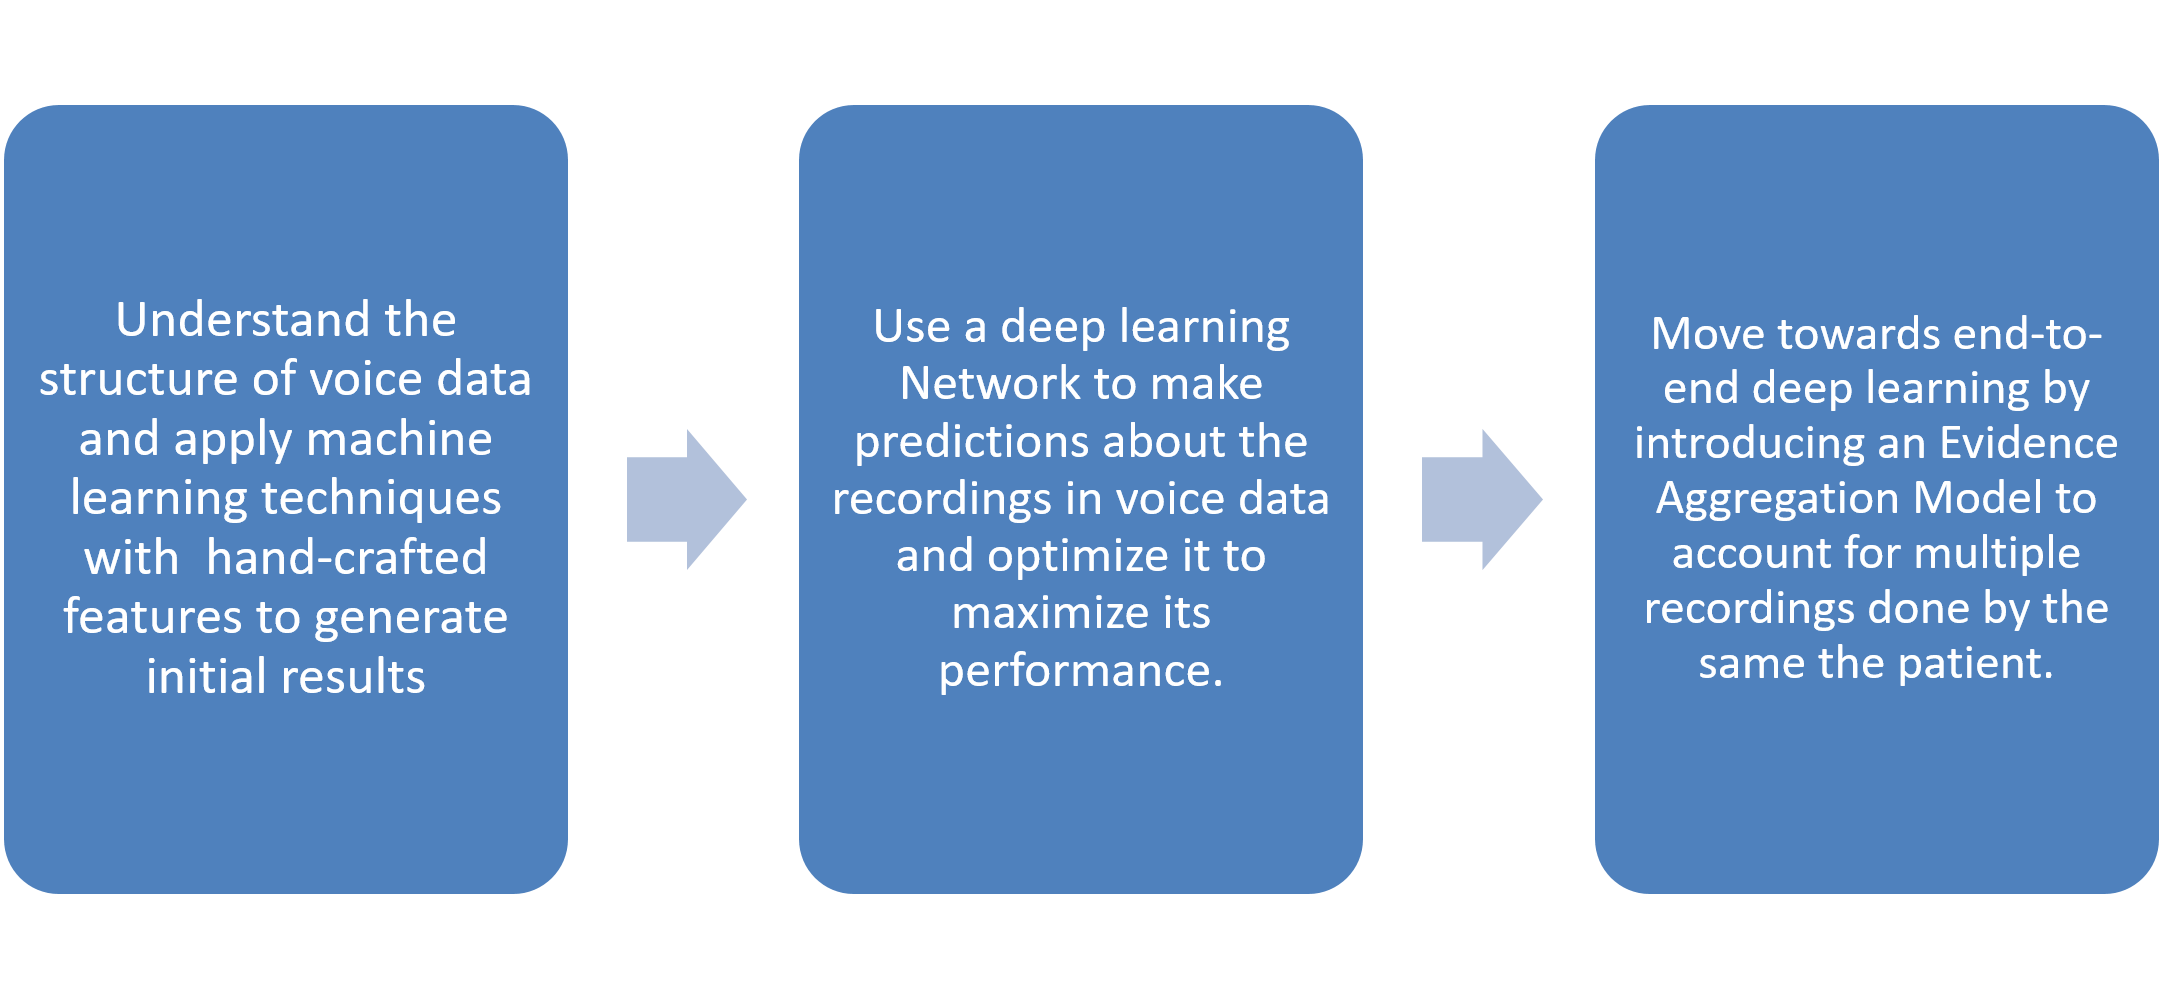
\includegraphics[width=\textwidth]{./Figures/park_method.png}
  \caption{System level design for Bioinformatics}
  \label{fig:park_method}
\end{figure}
\section{ Tools/Instruments}
\subsection{Simulation Software Packages}
We used the following sofwares/libraries for our applications:
\begin{itemize}
\item MATLAB
\item Python
\item Tensorflow
\item Keras
\item Scipy 
\item Numpy
\item Scikit-Learn
\end{itemize}
\subsection{Hardware Instruments}
We used \textbf{SOHRAB} Cluster at LUMS for our our simulation process. Its specifications are:\\
4 way SMP 48 Core E7-4830 v3 @ 2.10GHz, 256 GB RAM (Raid 10) 5*1.2 Tb - 3.3 Tb storage, Grid K40M GPU
